SyVOLT is a user-friendly Eclipse plugin to verify pre-/post- condition contracts on model transformations specified in the DSLTrans transformation language. The tool has a number of unique features, outlined below.

\subsection{Integration with Eclipse}

Providing our tool as an Eclipse plugin allows the user to work within a robust and popular development environment, while still allowing for easy setup of the prover. We are able to leverage the capabilities of Eclipse's graphical modelling evironments for artifact construction, as well as the Eclipse Generation Language (EGL) for the model-to-text production of required tool artifacts.

\subsection{Eclipse Frontend}
\begin{figure}
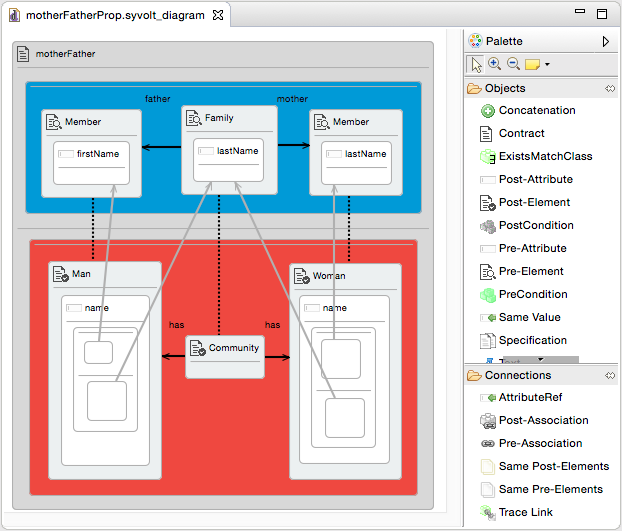
\includegraphics[width=0.45\textwidth]{figures/eclipse_frontend}
\caption{The transformation editor within Eclipse}
\label{fig:eclipse_frontend}
\end{figure}

Figure~\ref{fig:eclipse_frontend} shows the Eclipse frontend, where a user can edit a DSLTrans transformation within the Eclipse editor. A similar view is also used for users to define the contracts for their transformations. Note that these editors are based within the model creation framework FIX FIX.

\subsection{Graphical Modelling}
Both the transformation and the contracts are built using a graphical environment. This intuitive representation allows the user to quickly and easily visualize and construct the required contracts. This is in contrast to  the logical or mathematical expression approach which is required by other verification techniques.

\subsection{Handling of String Attributes}
The DSLTrans transformations and contracts are built upon typed graphs. 
Our contract prover is able to reason over these graphs to prove contracts. An example of this would be in the Families-To-Persons transformation from the ATL zoo [CITE]. In this transformation, the name for a person in the output graph is a concatenation of two strings from elements in the input graph.


\subsection{Import from ATL}
The ATL transformation language is commonly-used in both industry and academia. In order to support these users, we have developed a higher-order transformation that is able to automatically transform ATL transformations into our transformation language DSLTrans [CITE MODELS]. This allows the user to exhaustively prove contracts on ATL transformations.

\subsection{Push-Button Proving}
Once the transformation and the contracts of interest are created, one command can start the property proving process. This process will automatically create all required artifacts (as detailed in the following section), run the process, and then provide the results to the user within the Eclipse environment. This allows the user to continually stay within the Eclipse environment.

\subsection{Proving Speed}

Our technique is both valid and complete [CITE TECH REPORT], and will exhaustively prove whether a contract will hold for all possible input model to a transformation. However, our technique allows the proving process to take a relatively short amount of time. For example, our experiements on industrial transformations [CITE ATL] show that contracts can be verified within a few minutes. 

\subsection{Production of Counter-Examples}

An advantage of our technique is that a counter-example model for a particular contract is produced by the contract proving process. This allows the user to easily determine the error in the transformation and correct it. We suggest that these contracts be used analagous to 'test-driven development', in that development of a transformation is punctuated by contract proof.

\subsection{Input Independence and Exhaustiveness}

Our technique is valid and complete. Gives guaratnees over all input models for the transformation.

\subsection{Model-Driven Development}

Everything is modelled. Model transformations, and tooling.
 